\documentclass[a4paper,9pt]{article}

\usepackage[utf8]{inputenc}
\usepackage{graphicx}
\usepackage[francais]{babel}
%\usepackage{fullpage}
\usepackage{color}
\usepackage{array}
\usepackage{lstlisting}

\begin{document}


\begin{titlepage}
\centering
\huge
\bfseries
Visualisation Scientifique\\[1\baselineskip]
\vspace{0.5cm}
\normalfont
\large
Interpolation et Visualisation de données avec Paraview\\[1\baselineskip]
	
\vspace{2cm}

\begin{figure}[!h]
\centering
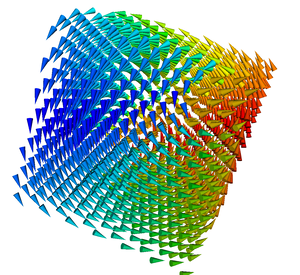
\includegraphics[width=0.9\textwidth]{couverture.png}
\end{figure}

\vspace{1.5cm}

\centering
\bfseries
\normalfont

\begin{tabular}{r c l}
Benjamin Aupetit & & Nicolas Cousin
\end{tabular}	

\vspace{0.5cm}

Ensimag\\
\textbf{\today}
\end{titlepage}

\clearpage
\newpage

\tableofcontents

\clearpage
\newpage

% INTRODUCTION

\section{Introduction}
\label{sec:introduction}
Une des étapes cruciales pour l'observation d'un phénomène a toujours été de prendre des séries de mesures des données physiques associées à ce phénomène. Malheureusement, il n'est pas toujours possible de mesurer une quantité en n'importe quel point de l'espace, d'abord parce que ça coûte cher et d'autre part parce que la position où l'on souhaite faire la mesure n'est pas toujours accessible.\\ Par conséquent, il existe des méthodes d'interpolation permettant d'évaluer approximativement la valeur d'une donnée physique (température, densité, ...) en un point de l'espace en fonction des valeurs que l'on a mesuré sur des positions voisines. Ce document présente deux méthodes d'interpolation que nous avons implémenté, et nous proposons ensuite de visualiser leurs résultats sur paraview qui est un logiciel permettant de visualiser les données d'une grille régulière.

\clearpage
\newpage

\section{Première Méthode : Shepard}
\label{sec:shepard}

\subsection{Description}
\label{subsec:shepard_description}
Le principe de cette méthode est de considérer que la valeur interpolée en une position de l'espace est une somme pondérée des valeurs des échantillons en entrée.
$$F(x)=\sum_{i=1}^{N} \omega_{i}(x).f_{i}$$
Chaque fonction de pondération $\omega_{i}$ est définie de la façon suivante :
$$\omega_{i}(x)=\frac{\prod_{j \neq i}^{N}[d_{j}(x)]^{\mu}}{\sum_{j=1}^{N} \prod_{k \neq j}^{N}[d_{k}(x)]^{\mu}} ~~~~~~ d_{i}(x)=||x-x_{i}||_{2}~~~,~~~\mu\ge1$$

\subsection{Complexité}
\label{subsec:shepard_complexite}
Notons $N$ le nombre d'échantillons de données en entrée et $R$ le produit des résolutions de la grille voulue :
$$R = resolution_{x}.resolution_{y}.resolution_{z}$$
La méthode de Shepard revient à multiplier deux matrices, l'une de taille $N.R$ qui contiendra à chaque ligne les différentes valeurs des coefficients $\omega_{i}$ pour un point de la grille, et l'autre étant le vecteur colonne de taille $N$ contenant les valeurs scalaires des échantillons en entrée. Le résultat de cette multiplication donne un vecteur colonne de taille $R$ contenant les $R$ valeurs scalaires interpolées pour les points de la grille.
$$S_{N,R}.F_{1,N}=Res_{1,R}$$
Le coût en calcul de cette méthode est donc la somme du coût pour construire la matrice S et le coût de la multiplication entre S et F.\\\\
\textbf{Coût de la construction de S}\\
Chaque coefficient de la matrice correspond au calcul d'un $\omega_{i}$ :
\begin{itemize}
\item Le coût de calcul du numérateur est en $O(N)$ mais doit être calculé pour chaque colonne d'une ligne de S
\item Le coût de calcul du dénominateur est en $O(N^{2})$ et peut être calculé une fois pour chaque ligne de S
\end{itemize}
Comme S a une largeur de $N$ et une hauteur de $R$, son coût de construction est donc en $O(N^{2}.R)$.\\\\
\textbf{Coût de la multiplication de S et F}\\
Etant donné la taille des matrices, son coût est en $O(N.R)$.\\\\
Par conséquent la méthode de Shepard a une complexité en \textbf{$O(N^{2}.R)$}.


\section{Deuxième Méthode : Multiquadriques de Hardy}
\label{sec:hardy}

\subsection{Description}
\label{subsec:hardy_description}
Cette méthode part du principe que la valeur interpolée en un point est le résultat de la multiplication de coefficients dont certains sont initialement inconnus.
$$F(x)=\sum_{k=1}^{N} \alpha_{k}.h_{k}(x)$$
Avec $h_{k}(x) = \sqrt{R+||x-x_{k}||^{2}}$ où $R$ est une constante.\\

Pour obtenir les valeurs interpolées des points sur une grille, il faut donc commencer par calculer la matrice des coefficients $\alpha_{k}$ puis la multiplier avec la matrice des $H_{k}$ qu'on aura construite pour les points à interpoler. Pour calculer la matrice des $\alpha_{k}$, nous avons choisi d'implémenter l'inversion de matrices par décomposition LU.

\subsection{Complexité}
\label{subsec:hardy_complexite}
Comme précèdemment, notons $N$ le nombre d'échantillons de données en entrée et $R$ le produit des résolutions de la grille voulue.
Dans cette méthode, nous calculons la matrice $H$ correspondant aux données et l'inversons. Ensuite nous obtenons la matrice des coefficients grâce au produit de la matrice inverse de $H$ et de la matrices contenant les valeurs des échantillons :
$$A_{1,N} = inv(H_{N,N}).F_{1,N}$$
Une fois que ces coefficients sont connus, l'on calcule la matrice H correspondant à la grille de points et on obtient le résultat par simple multiplication avec la matrice des coefficients :
$$H_{N,R}.A_{1,N}=Res_{1,R}$$
Le coût en calcul de cette méthode est donc égal à la somme des coûts de l'inversion d'une matrice carrée de taille N, des coûts de construction des deux matrices H et des coûts de multiplication de matrices.\\\\
\textbf{Coût d'inversion d'une matrice de taille N}\\
Le coût de l'inversion d'une matrice par la méthode de décomposition LU est en $O(N^{3})$.\\\\
\textbf{Coût de construction de H}\\
Comme le calcul de chaque coefficient de la matrice est en $O(1)$, le coût de construction de H est en $O(N^{2})$ pour la première (les données) et en $O(N.R)$ pour la seconde (les points de la grille).\\\\
\textbf{Coût des multiplications}\\
Les coûts des multiplications sont respectivement en $O(N^{2})$ pour $inv(H_{N,N}).F_{1,N}$ et $O(N.R)$ pour $H_{N,R}.A_{1,N}$.\\\\
Par conséquent la méthode de Hardy a une complexité en \textbf{$O(N.max(N^{2}.R))$}.


\section{Implémentation}
\label{sec:implementation}

\subsection{Types utilisés}
\label{subsec:types}
Nous avons choisi de développer notre application dans le langage C, par conséquent nous avons défini plusieurs types permettant de nous faciliter la tâche. Ainsi, une donnée est une structure contenant les coordonnées du point et sa valeur scalaire, un échantillon est un ensemble de données auquel on associe une bounding box, et un échantillon interpolé est composé uniquement d'un ensemble de scalaires et d'une bounding box.\\Il n'est en effet pas nécessaire de connaître les coordonnées des points dans un échantillon interpolé, car les positions sur la grille peuvent être facilement retrouvées à l'aide de la bounding box. Voici la description exacte de ces structures :

\begin{verbatim}
typedef double real;

struct _BoundingBox3D
{
	real xmin, xmax, ymin, ymax, zmin, zmax;
};
typedef struct _BoundingBox3D BoundingBox3D;

struct _Data3D 
{
	real x;
	real y;
	real z;
	real w;
};
typedef struct _Data3D Data3D;

struct _ScaterredData3D
{
	int           nbSamples;
	Data3D        *scaterred;
	BoundingBox3D obb;
};
typedef struct _ScaterredData3D ScaterredData3D;

struct _SampledData3D
{
	int           width;
	int           height;
	int           depth;
	BoundingBox3D obb;
	real          *sampledValue;
};
typedef struct _SampledData3D SampledData3D;
\end{verbatim}

\subsection{Implémentation de la méthode de Shepard}
\label{subsec:shepard_implementation}
Pour l'implémentation de Shepard, veuillez consulter les méthodes suivantes du fichier interpolate.c :
\begin{verbatim}
inline static real dist3sample(const Data3D a, const Data3D b);
inline static real computeWINom3(ScaterredData3D data, 
                                          Data3D X, int i);
inline static real sheparderp3(ScaterredData3D data, Data3D X);
void shepardInterpolation3D(GridType type, ScaterredData3D data,
                                          SampledData3D* result);
\end{verbatim}
La fonction dist3sample permet de retourner la distance entre 2 points de l'espace, et la fonction computeWINom3 permet de calculer le numérateur de $\omega_{i}(x)$. La majorité du travail est effectué par la fonction sheparderp3 qui calcule le denominateur de tous les $\omega_{i}(x)$ une seule fois et calcule leur numérateur pour chaque colonne. Cette fonction se charge aussi de faire la multiplication entre les $\omega_{i}(x)$ et les $f_{i}$.\\Enfin, la fonction shepardInterpolation3D s'occupe simplement d'appeler sheparderp3 sur chaque point de la grille à interpoler.\\Comme nous avons bien veillé à calculer le dénominateur des $\omega_{i}(x)$ une seule fois pour chaque x, notre implémentation a bien la complexité théorique de la méthode de Shepard : $O(N^{2}.R)$.

\subsection{Implémentation de la méthode des multiquadriques de Hardy}
\label{subsec:hardy_implementation}
Pour la méthode de Hardy, tout est implémenté dans une fonction unique :
\begin{verbatim}
void multiQuadricInterpolation3D(GridType type, 
                    ScaterredData3D data, SampledData3D *result);
\end{verbatim}
Cette fonction s'occupe de créer la première matrice H (les données) de manière à pouvoir l'inverser et obtenir la matrice des coefficients $\alpha_{i}$. Ensuite, l'on crée la seconde matrice H (les points de la grille) et obtenons les valeurs d'interpolation sur la grille.\\\\
L'inversion de matrice et la décomposition LU ont été implémentées dans le fichier matrix.c :
\begin{verbatim}
void LUfacto(Matrix mat, Matrix *L, Matrix *U);
Matrix* forwardLU(Matrix L, Matrix b);
Matrix* backwardLU(Matrix U, Matrix Y);
Matrix* invert(Matrix matrix);
\end{verbatim}
La fonction LUfacto permet de décomposer la matrice en un produit de 2 matrices $L$ et $U$ où L est triangulaire inférieure et $U$ est triangulaire supérieure. Une fois cette décomposition achevée, l'on peut résoudre facilement le système $$A.X=L.U.X=b$$ ForwardLU permet de résoudre le système $L.Y=b$ et backwardLU permet de résoudre le système $U.X=Y$. L'inversion de matrice correspond à la résolution du système $A.X=b$ où $b$ est la matrice identité, X sera donc l'inverse de $A$.\\
Nous avons bien sûr veillé à ce que notre implémentation respecte la complexité en $O(N^{3})$ de cette méthode de décomposition.

\section{Tests et Résultats}
\label{sec:tests_resultats}

\subsection{Visualisation de données avec Paraview}
\label{subsec:paraview}
Paraview est un logiciel permettant la visualisation de données sous forme d'une grille régulière. Il offre de nombreuses possibilités d'affichage, comme l'affichage de surfaces, de coupes d'un volume 3D, du volume 3D en transparence, ... Il permet en outre de customiser la carte de couleur utilisée pour représenter les valeurs scalaires associées aux points. Afin de pouvoir visualiser les données avec paraview, nous écrivons la grille résultat de l'interpolation dans un fichier portant l'extension 'vtk' que nous pouvons ensuite ouvrir depuis le logiciel. Cette fonction est présente dans le fichier data.c.
\begin{verbatim}
void ecrireFichierVTK3D(char *filePath, SampledData3D data);
\end{verbatim}

\subsection{Présentation des méthodes de tests}
\label{subsec:presentation_tests}
Afin de tester notre implémentation, nous avons commencé par tenter d'interpoler des données simples en 2D et 3D. Nous avons donc implémenté une fonction permettant de lire des données depuis un fichier ayant une syntaxe bien définie. Cette fonction est présente dans le fichier data.c et prend en entrée des fichiers ayant la syntaxe suivante :
\begin{verbatim}
// Nom de la fonction
ScaterredData3D* readData3D(char* fileName);

//Syntaxe du fichier

#DATA_DIMENSION
3

#NUMBER_POINTS
4

0.0 0.0 0.0
1.0 0.0 0.5
0.0 1.0 0.5
1.0 1.0 1.0
\end{verbatim}
L'entier DataDimension permet de définir combien de coordonnées aura chaque point, pour un point 2D, cet entier vaudra donc 3 (2 coordonnées + 1 scalaire). L'entier NumberPoints spécifie le nombre de points à lire dans le fichier. La fonction readData s'occupera d'allouer l'espace nécessaire au stockage de tout les points qui seront lus dans le fichier et d'enregistrer leurs coordonnées et scalaires.\\\\
Pour pouvoir pousser un peu plus loin l'analyse, nous avons aussi implémenté des fonctions permettant de générer des données de façon aléatoire à l'intérieur d'une bounding box. Dans la même optique, nous avons ajouté une fonction générant des coordonnées de points aléatoires, et un scalaire correspondant à leur sinus cardinal.
\begin{verbatim}
ScaterredData3D* generateRandomData3D(int nbSamples,
                                      real minX, real maxX,
                                      real minY, real maxY,
                                      real minZ, real maxZ,
                                      real minW, real maxW);
ScaterredData3D* generateSinCData3D(int nbSamples, real factor,
                                      real minX, real maxX,
                                      real minY, real maxY,
                                      real minZ, real maxZ);
\end{verbatim} 

\subsection{Validation de l'implémentation}
\label{subsec:validation_implementation}
\textbf{Validation de l'implémentation de Shepard}\\
\textbf{Validation de l'implémentation de Hardy}\\
Pour les mêmes fichiers en entrée que pour les tests de validation avec Shepard, nous obtenons les images ci dessous. Nous pouvons observer que les résultats d'interpolation semblent être excellents, il n'y a notamment pas les erreurs présentes sur l'interpolation diagonale de Shepard.
\begin{figure}[!h]
\centering
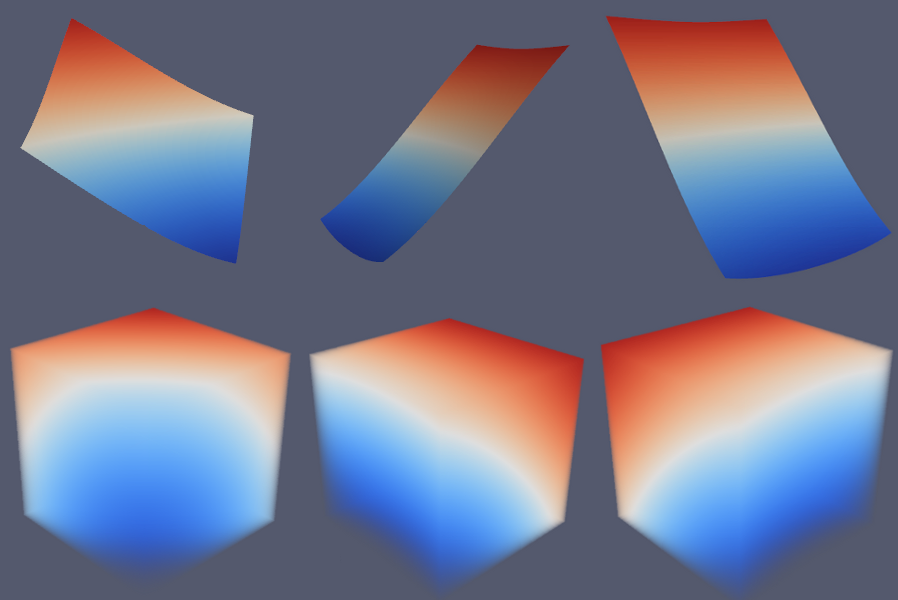
\includegraphics[width=0.9\textwidth]{images/multiquadric/tests_simples_mq.png}
\caption{Résultats des cas de tests simples avec méthode de Hardy}
\end{figure}


\subsection{Tests Complexes}
\label{subsec:tests_complexes}
Nous avons par la suite observé les résultats d'interpolation de ces deux méthodes sur des cas de tests plus poussés. Nous avons commencé par relever des données sur l'ensoleillement de plusieurs villes de France sur internet, voici les résultats que nous obtenons avec les 2 méthodes :

Un autre test 2D que nous avons effectué est celui du sinus cardinal que nous avions implémenté, les résultats sont bons quand on met assez d'échantillons, mais encore une fois, la méthode de Shepard laisse des artefacts qui dégradent la qualité de l'interpolation (flat points).

Ensuite, nous avons effectué le test des sinus cardinal en 3D pour les deux méthodes, on peut encore une fois observer les flat points de la méthode de Shepard et une très bonne approximation avec la méthode de Hardy.

Enfin, nous avons été chercher les valeurs moyennes de température minimale sur 103 villes de France sur 11 mois de l'année 2010 et avons effectué l'interpolation avec la méthode de Hardy. Quand nous avons voulu essayer de pratiquer la méthode de Shepard avec ces données, nous avons du abandonner car le résultat n'était toujours pas sorti 4 heures après le lancement de l'application. Voici ce que nous avons obtenu avec la méthode de Hardy :

\subsection{Comparaison des deux méthodes}
\label{subsec:comparaison_methodes}

\subsubsection{Temps de calcul}
\label{subsec:temps_calcul}
Nous avons effectué une comparaison des performances de la méthode de Shepard et Hardy sur plusieurs cas tests. Voici les résultats que nous obtenons :

\begin{tabular}{|c|c|c|c|}
\hline
Nombre echantillons & Résolution & Temps Shepard & Temps Hardy \\
\hline
44 & 100.100 (2D) & 4,2 s & \\
100 & 100.100 (2D) & 22,5 s & \\
100 & 100.100.100 (3D) & & \\
50 & 100.100.100 (3D) & & \\
100 & 50.50.50 (3D) & & \\
\hline
\end{tabular}

\subsubsection{Précision de l'interpolation}
\label{subsec:precision_interpolation}
Au vu des cas de tests que nous avons utilisé, il apparait que la méthode de Hardy est bien meilleure en général que la méthode de Shepard car elle évite d'avoir des 'flat' points. Le seul avantage qu'il pourrait y avoir à utiliser la méthode de Shepard serait dans le cas où l'on aurait $R<<N^{2}$, car la perte en précision serait justifiée par un gain en temps de calcul important.

\section{Conclusion}
\label{sec:conclusion}

\end{document}
